% !TEX encoding = UTF-8 Unicode
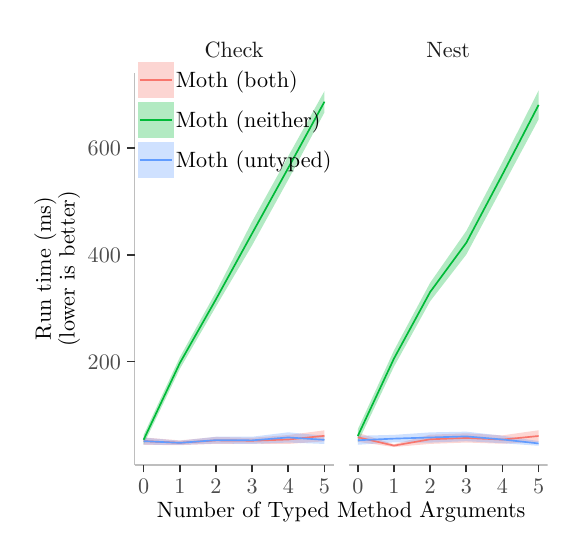
\begin{tikzpicture}[x=1pt,y=1pt]
\definecolor{fillColor}{RGB}{255,255,255}
\path[use as bounding box,fill=fillColor,fill opacity=0.00] (0,0) rectangle (187.90,180.67);
\begin{scope}
\path[clip] ( 38.64, 22.70) rectangle (110.52,164.42);
\definecolor{fillColor}{RGB}{248,118,109}

\path[fill=fillColor,fill opacity=0.30] ( 41.90, 32.61) --
	( 54.97, 31.53) --
	( 68.04, 32.78) --
	( 81.11, 32.49) --
	( 94.18, 33.47) --
	(107.25, 35.17) --
	(107.25, 31.20) --
	( 94.18, 30.26) --
	( 81.11, 30.34) --
	( 68.04, 30.30) --
	( 54.97, 29.81) --
	( 41.90, 29.93) --
	cycle;
\definecolor{fillColor}{RGB}{0,186,56}

\path[fill=fillColor,fill opacity=0.30] ( 41.90, 33.50) --
	( 54.97, 61.55) --
	( 68.04, 85.15) --
	( 81.11,110.64) --
	( 94.18,134.26) --
	(107.25,157.78) --
	(107.25,150.06) --
	( 94.18,125.76) --
	( 81.11,102.04) --
	( 68.04, 79.91) --
	( 54.97, 57.36) --
	( 41.90, 30.03) --
	cycle;
\definecolor{fillColor}{RGB}{97,156,255}

\path[fill=fillColor,fill opacity=0.30] ( 41.90, 32.55) --
	( 54.97, 31.41) --
	( 68.04, 32.86) --
	( 81.11, 32.85) --
	( 94.18, 34.46) --
	(107.25, 33.21) --
	(107.25, 30.25) --
	( 94.18, 30.75) --
	( 81.11, 30.25) --
	( 68.04, 30.38) --
	( 54.97, 29.90) --
	( 41.90, 29.98) --
	cycle;
\definecolor{drawColor}{RGB}{248,118,109}

\path[draw=drawColor,line width= 0.6pt,line join=round] ( 41.90, 31.27) --
	( 54.97, 30.67) --
	( 68.04, 31.54) --
	( 81.11, 31.41) --
	( 94.18, 31.86) --
	(107.25, 33.19);
\definecolor{drawColor}{RGB}{0,186,56}

\path[draw=drawColor,line width= 0.6pt,line join=round] ( 41.90, 31.76) --
	( 54.97, 59.45) --
	( 68.04, 82.53) --
	( 81.11,106.34) --
	( 94.18,130.01) --
	(107.25,153.92);
\definecolor{drawColor}{RGB}{97,156,255}

\path[draw=drawColor,line width= 0.6pt,line join=round] ( 41.90, 31.27) --
	( 54.97, 30.65) --
	( 68.04, 31.62) --
	( 81.11, 31.55) --
	( 94.18, 32.60) --
	(107.25, 31.73);
\end{scope}
\begin{scope}
\path[clip] (116.02, 22.70) rectangle (187.90,164.42);
\definecolor{fillColor}{RGB}{248,118,109}

\path[fill=fillColor,fill opacity=0.30] (119.29, 34.29) --
	(132.36, 30.15) --
	(145.43, 33.59) --
	(158.50, 34.09) --
	(171.56, 33.35) --
	(184.63, 35.20) --
	(184.63, 31.03) --
	(171.56, 30.32) --
	(158.50, 30.76) --
	(145.43, 30.27) --
	(132.36, 29.14) --
	(119.29, 31.03) --
	cycle;
\definecolor{fillColor}{RGB}{0,186,56}

\path[fill=fillColor,fill opacity=0.30] (119.29, 35.56) --
	(132.36, 64.04) --
	(145.43, 88.49) --
	(158.50,107.22) --
	(171.56,132.12) --
	(184.63,157.98) --
	(184.63,147.55) --
	(171.56,123.13) --
	(158.50, 98.68) --
	(145.43, 81.81) --
	(132.36, 58.18) --
	(119.29, 30.73) --
	cycle;
\definecolor{fillColor}{RGB}{97,156,255}

\path[fill=fillColor,fill opacity=0.30] (119.29, 33.21) --
	(132.36, 33.53) --
	(145.43, 34.43) --
	(158.50, 34.69) --
	(171.56, 33.22) --
	(184.63, 31.27) --
	(184.63, 29.59) --
	(171.56, 30.50) --
	(158.50, 31.25) --
	(145.43, 30.74) --
	(132.36, 30.82) --
	(119.29, 29.95) --
	cycle;
\definecolor{drawColor}{RGB}{248,118,109}

\path[draw=drawColor,line width= 0.6pt,line join=round] (119.29, 32.66) --
	(132.36, 29.65) --
	(145.43, 31.93) --
	(158.50, 32.42) --
	(171.56, 31.83) --
	(184.63, 33.12);
\definecolor{drawColor}{RGB}{0,186,56}

\path[draw=drawColor,line width= 0.6pt,line join=round] (119.29, 33.14) --
	(132.36, 61.11) --
	(145.43, 85.15) --
	(158.50,102.95) --
	(171.56,127.63) --
	(184.63,152.77);
\definecolor{drawColor}{RGB}{97,156,255}

\path[draw=drawColor,line width= 0.6pt,line join=round] (119.29, 31.58) --
	(132.36, 32.17) --
	(145.43, 32.59) --
	(158.50, 32.97) --
	(171.56, 31.86) --
	(184.63, 30.43);
\end{scope}
\begin{scope}
\path[clip] ( 38.64,164.42) rectangle (110.52,180.67);
\definecolor{drawColor}{gray}{0.10}

\node[text=drawColor,anchor=base,inner sep=0pt, outer sep=0pt, scale=  0.80] at ( 74.58,169.79) {Check};
\end{scope}
\begin{scope}
\path[clip] (116.02,164.42) rectangle (187.90,180.67);
\definecolor{drawColor}{gray}{0.10}

\node[text=drawColor,anchor=base,inner sep=0pt, outer sep=0pt, scale=  0.80] at (151.96,169.79) {Nest};
\end{scope}
\begin{scope}
\path[clip] (  0.00,  0.00) rectangle (187.90,180.67);
\definecolor{drawColor}{RGB}{190,190,190}

\path[draw=drawColor,line width= 0.6pt,line join=round] ( 38.64, 22.70) --
	(110.52, 22.70);
\end{scope}
\begin{scope}
\path[clip] (  0.00,  0.00) rectangle (187.90,180.67);
\definecolor{drawColor}{gray}{0.20}

\path[draw=drawColor,line width= 0.6pt,line join=round] ( 41.90, 19.95) --
	( 41.90, 22.70);

\path[draw=drawColor,line width= 0.6pt,line join=round] ( 54.97, 19.95) --
	( 54.97, 22.70);

\path[draw=drawColor,line width= 0.6pt,line join=round] ( 68.04, 19.95) --
	( 68.04, 22.70);

\path[draw=drawColor,line width= 0.6pt,line join=round] ( 81.11, 19.95) --
	( 81.11, 22.70);

\path[draw=drawColor,line width= 0.6pt,line join=round] ( 94.18, 19.95) --
	( 94.18, 22.70);

\path[draw=drawColor,line width= 0.6pt,line join=round] (107.25, 19.95) --
	(107.25, 22.70);
\end{scope}
\begin{scope}
\path[clip] (  0.00,  0.00) rectangle (187.90,180.67);
\definecolor{drawColor}{gray}{0.30}

\node[text=drawColor,anchor=base,inner sep=0pt, outer sep=0pt, scale=  0.80] at ( 41.90, 12.24) {0};

\node[text=drawColor,anchor=base,inner sep=0pt, outer sep=0pt, scale=  0.80] at ( 54.97, 12.24) {1};

\node[text=drawColor,anchor=base,inner sep=0pt, outer sep=0pt, scale=  0.80] at ( 68.04, 12.24) {2};

\node[text=drawColor,anchor=base,inner sep=0pt, outer sep=0pt, scale=  0.80] at ( 81.11, 12.24) {3};

\node[text=drawColor,anchor=base,inner sep=0pt, outer sep=0pt, scale=  0.80] at ( 94.18, 12.24) {4};

\node[text=drawColor,anchor=base,inner sep=0pt, outer sep=0pt, scale=  0.80] at (107.25, 12.24) {5};
\end{scope}
\begin{scope}
\path[clip] (  0.00,  0.00) rectangle (187.90,180.67);
\definecolor{drawColor}{RGB}{190,190,190}

\path[draw=drawColor,line width= 0.6pt,line join=round] (116.02, 22.70) --
	(187.90, 22.70);
\end{scope}
\begin{scope}
\path[clip] (  0.00,  0.00) rectangle (187.90,180.67);
\definecolor{drawColor}{gray}{0.20}

\path[draw=drawColor,line width= 0.6pt,line join=round] (119.29, 19.95) --
	(119.29, 22.70);

\path[draw=drawColor,line width= 0.6pt,line join=round] (132.36, 19.95) --
	(132.36, 22.70);

\path[draw=drawColor,line width= 0.6pt,line join=round] (145.43, 19.95) --
	(145.43, 22.70);

\path[draw=drawColor,line width= 0.6pt,line join=round] (158.50, 19.95) --
	(158.50, 22.70);

\path[draw=drawColor,line width= 0.6pt,line join=round] (171.56, 19.95) --
	(171.56, 22.70);

\path[draw=drawColor,line width= 0.6pt,line join=round] (184.63, 19.95) --
	(184.63, 22.70);
\end{scope}
\begin{scope}
\path[clip] (  0.00,  0.00) rectangle (187.90,180.67);
\definecolor{drawColor}{gray}{0.30}

\node[text=drawColor,anchor=base,inner sep=0pt, outer sep=0pt, scale=  0.80] at (119.29, 12.24) {0};

\node[text=drawColor,anchor=base,inner sep=0pt, outer sep=0pt, scale=  0.80] at (132.36, 12.24) {1};

\node[text=drawColor,anchor=base,inner sep=0pt, outer sep=0pt, scale=  0.80] at (145.43, 12.24) {2};

\node[text=drawColor,anchor=base,inner sep=0pt, outer sep=0pt, scale=  0.80] at (158.50, 12.24) {3};

\node[text=drawColor,anchor=base,inner sep=0pt, outer sep=0pt, scale=  0.80] at (171.56, 12.24) {4};

\node[text=drawColor,anchor=base,inner sep=0pt, outer sep=0pt, scale=  0.80] at (184.63, 12.24) {5};
\end{scope}
\begin{scope}
\path[clip] (  0.00,  0.00) rectangle (187.90,180.67);
\definecolor{drawColor}{RGB}{190,190,190}

\path[draw=drawColor,line width= 0.6pt,line join=round] ( 38.64, 22.70) --
	( 38.64,164.42);
\end{scope}
\begin{scope}
\path[clip] (  0.00,  0.00) rectangle (187.90,180.67);
\definecolor{drawColor}{gray}{0.30}

\node[text=drawColor,anchor=base east,inner sep=0pt, outer sep=0pt, scale=  0.80] at ( 33.69, 57.27) {200};

\node[text=drawColor,anchor=base east,inner sep=0pt, outer sep=0pt, scale=  0.80] at ( 33.69, 95.85) {400};

\node[text=drawColor,anchor=base east,inner sep=0pt, outer sep=0pt, scale=  0.80] at ( 33.69,134.42) {600};
\end{scope}
\begin{scope}
\path[clip] (  0.00,  0.00) rectangle (187.90,180.67);
\definecolor{drawColor}{gray}{0.20}

\path[draw=drawColor,line width= 0.6pt,line join=round] ( 35.89, 60.03) --
	( 38.64, 60.03);

\path[draw=drawColor,line width= 0.6pt,line join=round] ( 35.89, 98.60) --
	( 38.64, 98.60);

\path[draw=drawColor,line width= 0.6pt,line join=round] ( 35.89,137.17) --
	( 38.64,137.17);
\end{scope}
\begin{scope}
\path[clip] (  0.00,  0.00) rectangle (187.90,180.67);
\definecolor{drawColor}{RGB}{0,0,0}

\node[text=drawColor,anchor=base,inner sep=0pt, outer sep=0pt, scale=  0.80] at (113.27,  3.82) {Number of Typed Method Arguments};
\end{scope}
\begin{scope}
\path[clip] (  0.00,  0.00) rectangle (187.90,180.67);
\definecolor{drawColor}{RGB}{0,0,0}

\node[text=drawColor,rotate= 90.00,anchor=base,inner sep=0pt, outer sep=0pt, scale=  0.80] at (  8.36, 93.56) {Run time (ms)};

\node[text=drawColor,rotate= 90.00,anchor=base,inner sep=0pt, outer sep=0pt, scale=  0.80] at ( 17.00, 93.56) {(lower is better)};
\end{scope}
\begin{scope}
\path[clip] (  0.00,  0.00) rectangle (187.90,180.67);
\definecolor{fillColor}{RGB}{255,255,255}

\path[fill=fillColor] ( 39.13,154.64) rectangle ( 53.58,169.10);
\end{scope}
\begin{scope}
\path[clip] (  0.00,  0.00) rectangle (187.90,180.67);
\definecolor{fillColor}{RGB}{248,118,109}

\path[fill=fillColor,fill opacity=0.30] ( 39.84,155.35) rectangle ( 52.87,168.38);
\end{scope}
\begin{scope}
\path[clip] (  0.00,  0.00) rectangle (187.90,180.67);
\definecolor{drawColor}{RGB}{248,118,109}

\path[draw=drawColor,line width= 0.6pt,line join=round] ( 40.57,161.87) -- ( 52.14,161.87);
\end{scope}
\begin{scope}
\path[clip] (  0.00,  0.00) rectangle (187.90,180.67);
\definecolor{fillColor}{RGB}{255,255,255}

\path[fill=fillColor] ( 39.13,140.19) rectangle ( 53.58,154.64);
\end{scope}
\begin{scope}
\path[clip] (  0.00,  0.00) rectangle (187.90,180.67);
\definecolor{fillColor}{RGB}{0,186,56}

\path[fill=fillColor,fill opacity=0.30] ( 39.84,140.90) rectangle ( 52.87,153.93);
\end{scope}
\begin{scope}
\path[clip] (  0.00,  0.00) rectangle (187.90,180.67);
\definecolor{drawColor}{RGB}{0,186,56}

\path[draw=drawColor,line width= 0.6pt,line join=round] ( 40.57,147.42) -- ( 52.14,147.42);
\end{scope}
\begin{scope}
\path[clip] (  0.00,  0.00) rectangle (187.90,180.67);
\definecolor{fillColor}{RGB}{255,255,255}

\path[fill=fillColor] ( 39.13,125.73) rectangle ( 53.58,140.19);
\end{scope}
\begin{scope}
\path[clip] (  0.00,  0.00) rectangle (187.90,180.67);
\definecolor{fillColor}{RGB}{97,156,255}

\path[fill=fillColor,fill opacity=0.30] ( 39.84,126.45) rectangle ( 52.87,139.48);
\end{scope}
\begin{scope}
\path[clip] (  0.00,  0.00) rectangle (187.90,180.67);
\definecolor{drawColor}{RGB}{97,156,255}

\path[draw=drawColor,line width= 0.6pt,line join=round] ( 40.57,132.96) -- ( 52.14,132.96);
\end{scope}
\begin{scope}
\path[clip] (  0.00,  0.00) rectangle (187.90,180.67);
\definecolor{drawColor}{RGB}{0,0,0}

\node[text=drawColor,anchor=base west,inner sep=0pt, outer sep=0pt, scale=  0.80] at ( 53.58,159.11) {Moth (both)};
\end{scope}
\begin{scope}
\path[clip] (  0.00,  0.00) rectangle (187.90,180.67);
\definecolor{drawColor}{RGB}{0,0,0}

\node[text=drawColor,anchor=base west,inner sep=0pt, outer sep=0pt, scale=  0.80] at ( 53.58,144.66) {Moth (neither)};
\end{scope}
\begin{scope}
\path[clip] (  0.00,  0.00) rectangle (187.90,180.67);
\definecolor{drawColor}{RGB}{0,0,0}

\node[text=drawColor,anchor=base west,inner sep=0pt, outer sep=0pt, scale=  0.80] at ( 53.58,130.21) {Moth (untyped)};
\end{scope}
\end{tikzpicture}
